\documentclass{article}
\usepackage{graphicx}
\usepackage{listings}
\usepackage{color}
\usepackage{amsmath}
\usepackage{amsfonts}
\usepackage{bm}
\usepackage[utf8]{inputenc}

\title{Metodi numerici\\
	Corso di LSMC, a.a. 2017-2018}
\author{Davide Gori\\
	550282}


\definecolor{backcolour}{rgb}{0.95,0.95,0.92}
\definecolor{gray}{rgb}{0.5,0.5,0.5}
\lstset{basicstyle=\ttfamily\small,
	columns=fullflexible,
	numbers=left,
	numberstyle=\tiny\ttfamily\color{gray},
	backgroundcolor=\color{backcolour},
	tabsize=4,
	language=Octave
}


\begin{document}
	\maketitle
	\section{Prima sperimentazione: un classico problema}
	Considero il seguente problema:
	\begin{equation}
	\begin{cases}
	y'=-y, & x \in \left(0, 10\right] \\
	y(0)=1
	\end{cases}
	\end{equation}
	la cui soluzione esatta è: $y(x) = e^{-x}$.
	Risolvo numericamente il problema mediante il metodo di Eulero. e utilizzando il comando subplot, suddivido un figura in quattro parti. In ciascuna di esse disegno la soluzione esatta e la soluzione numerica ottenuta per i valori del passo di integrazione $h = 0.5, 1, 2, 2.5$, rispettivamente. In ciascun grafico identifico le soluzioni disegnate utilizzando il comando legend.
	\subsection{Il codice}
	Questo è lo script che realizza la sperimentazione:
	
	\lstinputlisting{LabSper_2_1.m}
	
	Dove {\tt fun2.m} è la seguente:
	
	\lstinputlisting{fun2.m}
	\subsection{Risultati}
	
	Riportiamo il grafico in output.
	
	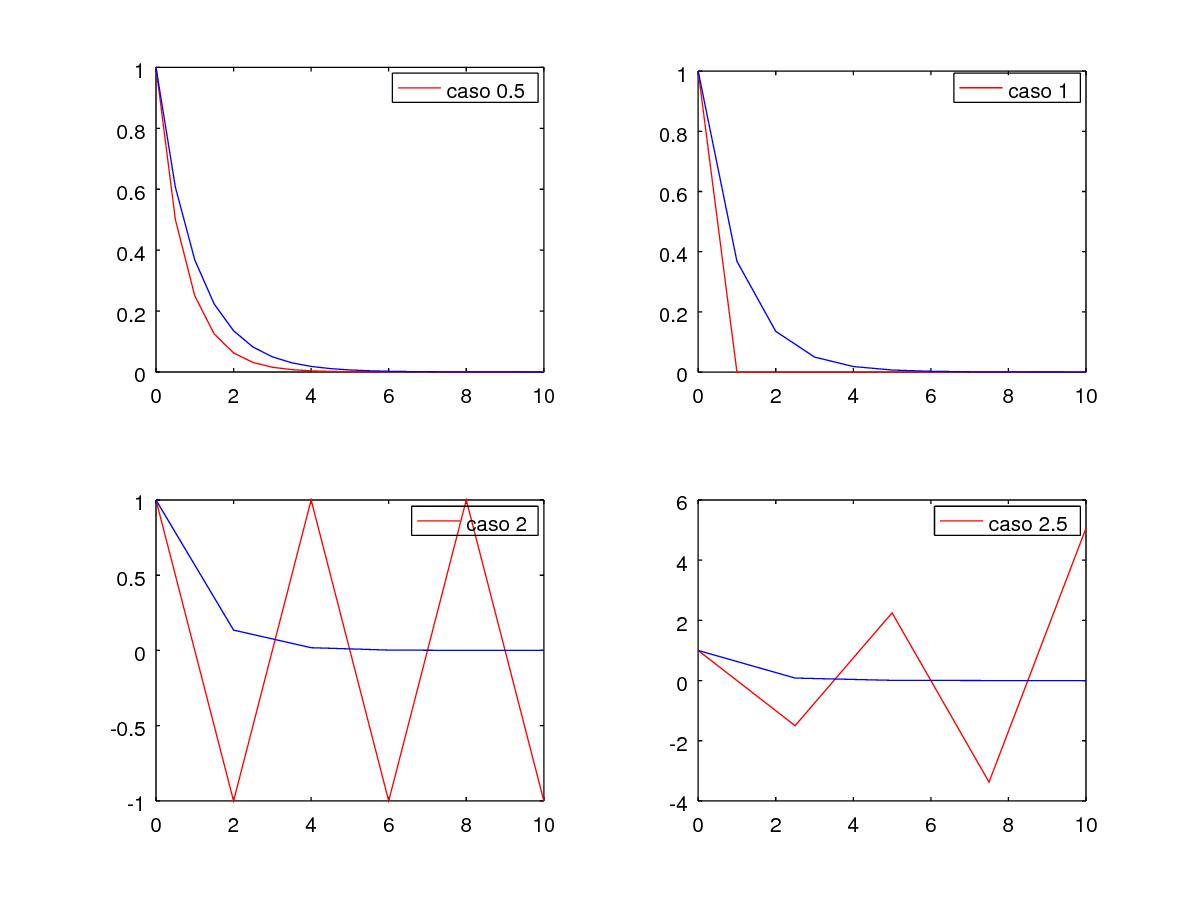
\includegraphics[width=\textwidth]{2_1_confronto_h.jpeg}
	
	Se uso un passo troppo grande ottengo che la funzione esce da [0, 1] e si ha un comportamento a "zig-zag" dovuto al fatto che la derivata cambia segno ad ogni passo
	
	\section{Seconda sperimentazione: metodo di Runge-Kutta}
	Scriviamo un file di tipo function che implementi su una griglia uniforme il metodo di Runge-Kutta classico per la risoluzione del problema ai valori iniziali:
	\begin{equation}
	\begin{cases}
	\bm{y'}=\bm{f}(x,\bm{y}), & x \in\left[x_0, T\right] \\
	y(x_0)=y_0
	\end{cases}
	\end{equation}
	con $\bm{f} : \mathbb{R} \times \mathbb{R}^n \rightarrow \mathbb{R}^n$. \\
	Applicheremo poi la function { \tt RK4.m} al problema precedente, con h = 1, 2, 2.5, 3.

	\subsection{Il codice}
	Questa è la funzione {\tt RK4.m}:
	
	\lstinputlisting{RK4.m}
	
	Questo è lo script che risolve il problema precedente con il metodo di Runge-Kutta:
	
	\lstinputlisting{LabSper_2_2.m}
	
	Dove {\tt fun2.m} è la seguente:
	
	\lstinputlisting{fun2.m}
	\subsection{Risultati}
	
	Riportiamo il grafico in output.
	
	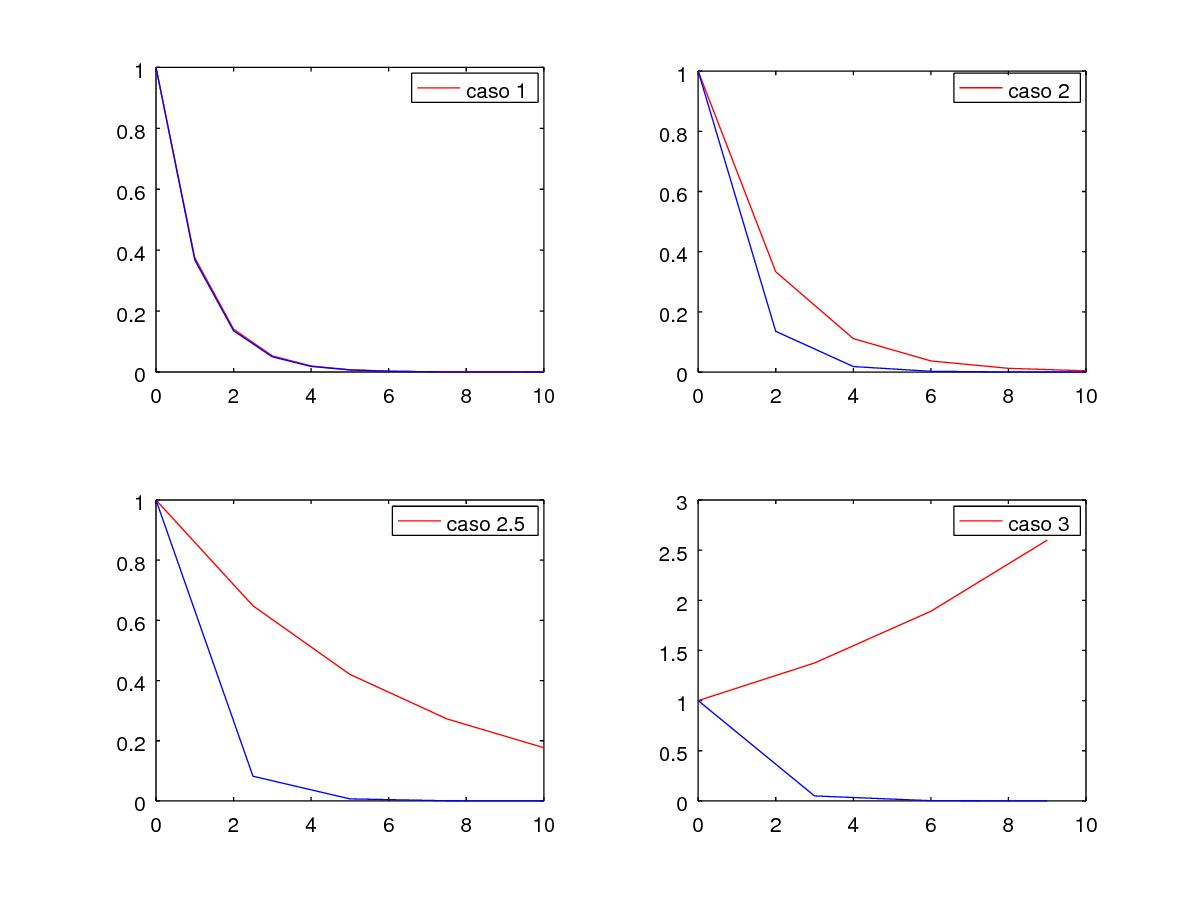
\includegraphics[width=\textwidth]{2_2_confronto_h_RK.jpeg}
	
	Si nota che usando RK4 la soluzione è più precisa, in 
	particolare non si verifica il fenomeno "zig-zag" che accadeva nella precedente sperimentazione.
	
	\section{Terza sperimentazione: applicazione di Runge-Kutta}
	Risolviamo con il metodo di Runge-Kutta classico il seguente problema ai valori iniziali:
	\begin{equation}
	\begin{cases}
	y''=-\frac{4x+1}{2(x+1)} y'+ \frac{2x-1}{4x^2} \cdot \frac{3y^3+y}{y^2+1}, & x \in\left[1, 2\right] \\
	y'(1)=1 \\
	y(1)=0
	\end{cases}
	\end{equation}
	Applicheremo poi la function { \tt RK4.m} con $h=0.01$.
	
	\subsection{Il codice}
	
	Questo è lo script che risolve il problema con il metodo di Runge-Kutta:
	
	\lstinputlisting{LabSper_2_3.m}
	
	Dove {\tt fun3.m} è la seguente:
	
	\lstinputlisting{fun3.m}
	\subsection{Risultati}
	
	Riportiamo il grafico in output.
	
	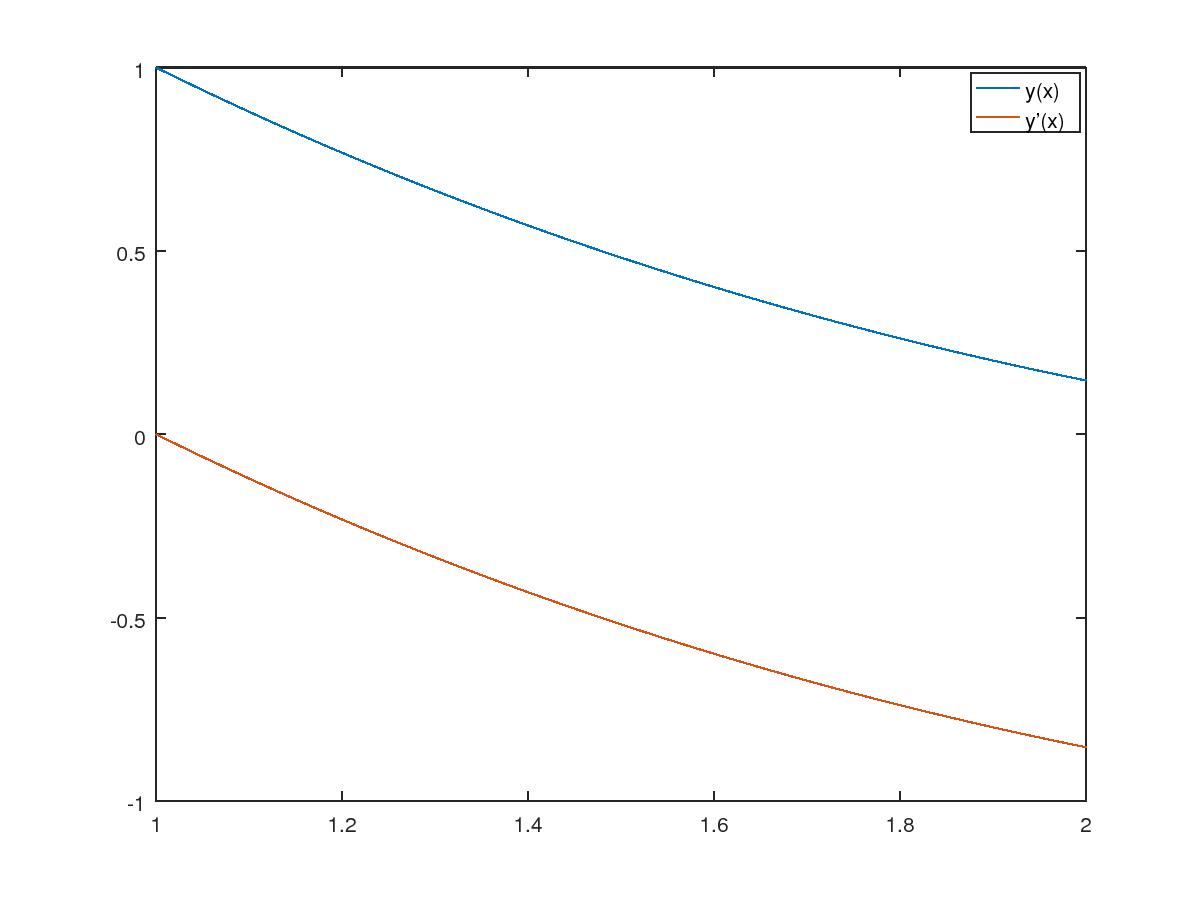
\includegraphics[width=\textwidth]{2_3_soluzione.jpeg}
	
	\section{Quarta sperimentazione: confronto tra Runge-Kutta e Eulero}
	Consideriamo il seguente problema ai valori iniziali:
	\begin{equation}
	\begin{cases}
	y'=-y-5e^{-t} \sin(5t), & x \in\left[0, 5\right] \\
	y(0)=1
	\end{cases}
	\end{equation}
	la cui soluzione esatta è $y=e^{-t} \cos(5t)$.
	Stimeremo l’ordine di convergenza sia del metodo di Eulero che del metodo di RungeKutta classico, calcolando l’errore commesso per $h=\frac{1}{10k}$ con $k = 1, \dots , 10$. Rappresentando gli errori in un grafico opportuno.
	
	\subsection{Il codice}
	Questo è lo script che risolve il problema precedente con il metodo di Runge-Kutta:
	
	\lstinputlisting{LabSper_2_4.m}
	
	Dove {\tt fun4.m} è la seguente:
	
	\lstinputlisting{fun4.m}
	\subsection{Risultati}
	\begin{figure}[htp!]
		\centering 
		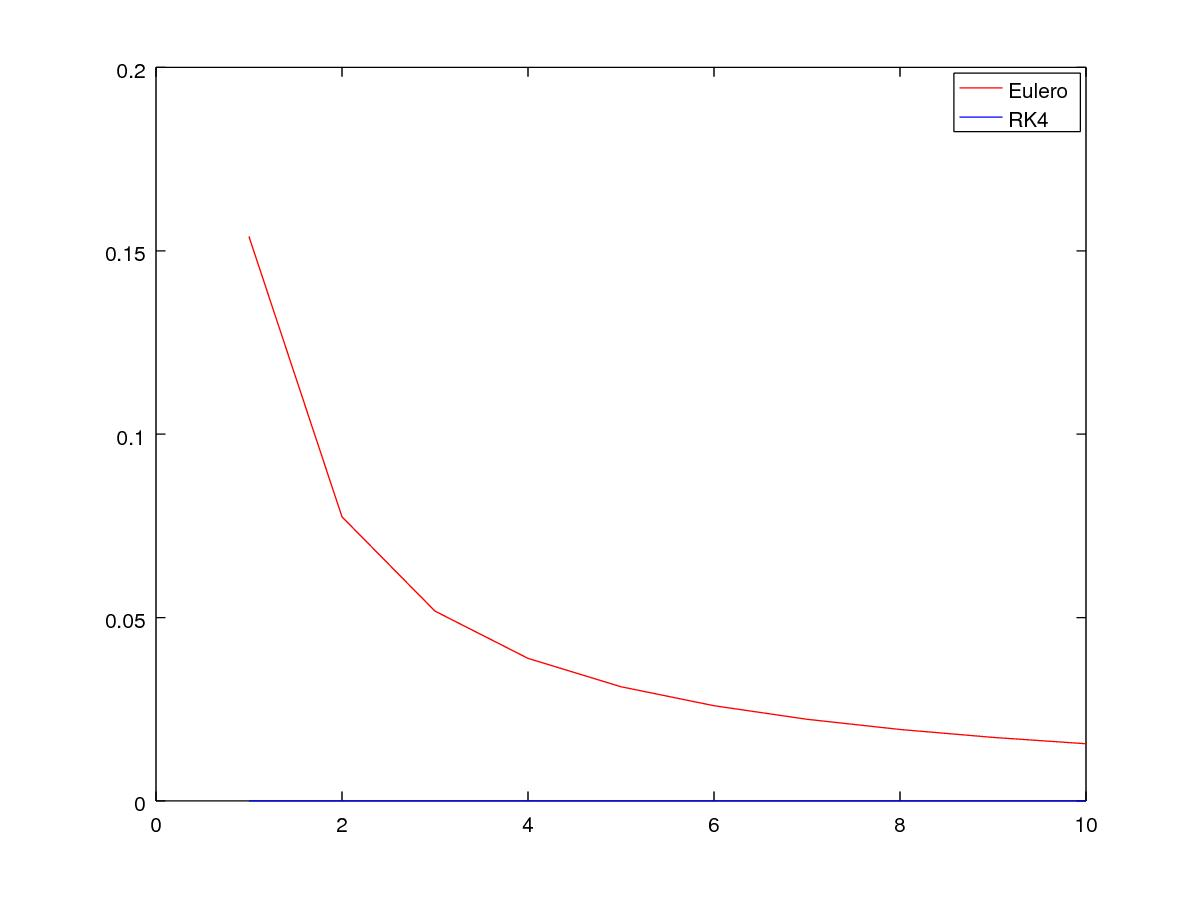
\includegraphics[width=0.7\textwidth]{2_4_confronto_RK_eulero.jpeg}
	\end{figure}

	Riportiamo il grafico in output.
	Notiamo che il metodo di Eulero è molto meno preciso di RK4.
	
	\begin{tabular}{|l|l|l|}
	\hline
	i & eulero & RK4 \\ \hline
	i=1 & 1.5386e-01 & 2.3929e-05 \\ \hline
	i=2 & 7.7457e-02 & 1.4690e-06 \\ \hline
	i=3 & 5.1750e-02 & 2.8876e-07 \\ \hline
	i=4 & 3.8870e-02 & 9.1275e-08 \\ \hline
	i=5 & 3.1132e-02 & 3.7356e-08 \\ \hline
	i=6 & 2.5960e-02 & 1.8002e-08 \\ \hline
	i=7 & 2.2259e-02 & 9.7114e-09 \\ \hline
	i=8 & 1.9481e-02 & 5.6899e-09 \\ \hline
	i=9 & 1.7319e-02 & 3.5508e-09 \\ \hline
	i=10 & 1.5589e-02 & 2.3294e-09 \\ \hline
	\end{tabular}

	\section{Sesta sperimentazione: confronto tra metodi numerici}
	Fissato $h = 0.1, 0.01, 0.001$, calcolo l’errore relativo e l’errore assoluto che si commettono nell’approssimare con il metodo di Eulero i due problemi ai valori iniziali
	\begin{equation}
	\begin{cases}
	y'(x)=-\alpha y +2x, & x \in\left[0, 6\right] \\
	y(0)=1
	\end{cases}
	\end{equation}
	ottenuti per $1\alpha= 1$ e $\alpha = 100$, sapendo che la soluzione esatta è
	$$y=\left(1+\frac{2}{\alpha^2}\right) e^{-\alpha x}+ \frac{2}{\alpha} x-\frac{2}{\alpha^2}$$
	Confronterò poi gli errori ottenuti con quelli applicando la routine {\tt ode45} con {\tt RelTol=10-7}. Inoltre, per entrambi i valori di $\alpha$, rappresenterò in un grafico il passo di integrazione adattivo determinato da {\tt ode45}.
	\subsection{Il codice}
	Questo è lo script usato:
	
	\lstinputlisting{LabSper_2_6.m}
	
	Dove {\tt fun4.m} è la seguente:
	
	\lstinputlisting{fun4.m}
	\subsection{Risultati}
	
	Riportiamo il grafico in output.
	
	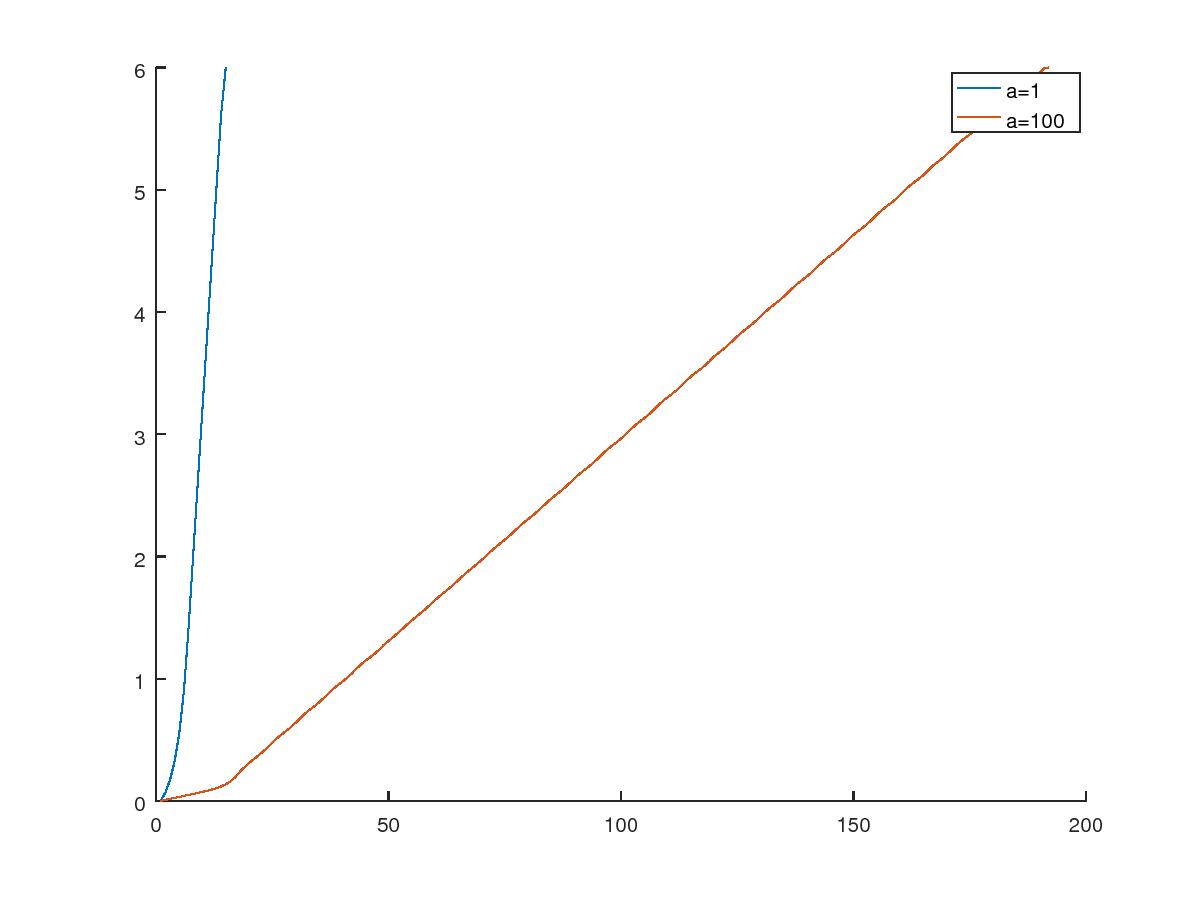
\includegraphics[width=\textwidth]{2_6.jpeg}
	Confronto con ode45: notiamo che il metodo di Eulero è molto meno preciso di ode45. \\
	I valori sono i seguenti:\\
	Errore assoluto:\\
	\begin{tabular}{|l|l|l|}
		\hline
		 h & a=1 & a=100 \\ \hline
		h=E-1 & 5.7603e-02 & 1.7974e+57 \\ \hline
		h=E-2 & 5.5413e-03 & 3.6795e-01 \\ \hline
		h=E-3 & 5.5205e-04 & 1.9205e-02 \\ \hline
		ode45 & 1.8360e-05 & 2.5751e-04 \\ \hline
	\end{tabular}\\
	Errore relativo:\\
	\begin{tabular}{|l|l|l|}
		\hline
		h & a=1 & a=100 \\ \hline
		h=E-1 & 6.1663e-02 & 1.5003e+58 \\ \hline
		h=E-2 & 5.9073e-03 & 1.0000e+00 \\ \hline
		h=E-3 & 5.8806e-04 & 2.1113e-01 \\ \hline
		ode45 & 7.5516e-06 & 1.8043e-03 \\ \hline
	\end{tabular}
	\\
	Passo ode45: Notiamo che nel caso a=100, escluso il momento iniziale, si ha che il passo è costante. Nel caso a=1 vengono eseguiti meno passi (15) ma più lunghi

	

\end{document}